\chapter{Porting BaseX to the Android platform}
\label{sec:migration:porting-basex-to-android}
In this chapter it is shown how the BaseX database has been migrated to the Android platform.
To achieve this goal the source and target platforms are analyzed and all requirements are determined.
The main focus here is on the different software platforms and not the hardware specific aspects because of the big variety of systems. 
In Section~\ref{sec:migration:problems-during-the-migration} it is illustrated which parts of the BaseX version has been changed and how to receive a working BaseX Android version.
The last section describes the problems which are occurred during the migration of the database to Android.


\section{Analyzing the source and target platforms} 
\label{sec:migration:analysing-the-source-and-target-platform}
In this section the two different platforms are analyzed.
The main part of it is the software part, because both platforms are running on a huge amount of hardware devices.
The source platform is the Java Virtual Machine (JVM) and the target platform is the Dalvik Virtual Machine (Dalvik VM, or DVM) in the Android environment.
The JVM and the DVM are both virtual machines (VM), but they vary in different ways.
A virtual machine is a simulated computer, which can be a whole system with all parts a computer provides.
Or it is an abstraction layer which provides the functionality to execute a program on every system that runs the virtual machine.
Unlike compiled machine code a program for a virtual machine is platform independent, because it does not matter on which operating system it is executed, as long as the virtual machine is available.
A disadvantage of this is the loss of speed, which is a result of the execution of the virtual machine and not only the program in general.~\cite{craig2006virtual}
\\
For both virtual machines the programming language Java is used, which is being compiled into code that the VMs understand and are able to execute.
Although both platforms are virtual machines they differ in some crucial ways.
One of the main difference is that the JVM is a stack based and the DVM is a register based virtual machine.
Also the DVM is optimized to be executed on mobile devices, which means that it is designed to use less memory and CPU usage than the JVM.
Lesser hardware usage implies also lesser battery usage, which is also a factor which should be considered in the field of mobile development.
Another difference which need to be considered is the host system, which is in the DVM case Android.
And on the opposite to this it could be Windows, Mac OS, or any Linux/Unix derivate for the JVM. 
This need to be considered if external sources will be used, like writing or reading a file.


\subsection{Comparison of the two virtual machines}
\label{sec:migration:comparison-of-the-two-virtual-machines}
Like in the chapter before mentioned both source and target platforms are using Java as a programming language.
Compared to other general purpose programming languages, for example C++, Java is not being compiled into machine code.
To execute Java code a virtual machine is required, which runs the compiled Java code.
However, like in Section~\ref{sec:migration:analysing-the-source-and-target-platform} mentioned both platforms have different virtual machines.
They differ in many kinds that the application developer not sees but need to consider.
\\
On of the most important difference is that the JVM is stack and the DVM is a register based virtual machine.
This difference helps the DVM to execute the same code in lesser operations than the JVM.
This means that the DVM need lesser CPU cycles than the JVM, which is an improvement that is necessary because of the lack of CPU resources in mobile devices and the aspect of the battery usage.
This can be demonstrated by looking at the instructions done by adding two integers.
The stack based virtual machine has to do four machine instructions, while the register based VM can do the operation in one instruction.
The reason for this is that the stack based VM needs to pop the two values first before it can add and store them back on the stack.
The instructions are \textit{pop 1, pop 2, add 1 2, push result}.\\
Figure~\ref{fig:stack-based-addition} illustrates the executed instructions of a addition with a stack based virtual machine.
\begin{figure}[h]
\begin{center}
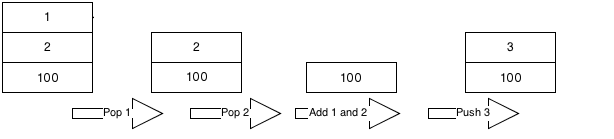
\includegraphics[scale=0.65]{images/stack-based-addition.png} 
\caption{The addition of two integers on a stack based virtual machine.}
\label{fig:stack-based-addition}
\end{center}
\end{figure}

Compared to this, the register based virtual machine just need one machine instruction to complete the same addition of two numbers.
The needed instruction is \textit{ADD R1, R2, R3}, which can be translated into add content of register 1 and register 2 and store it in register 3.
Figure~\ref{fig:register-based-addition} illustrates this by showing the add operation of the numbers one and two.
\begin{figure}[h]
\begin{center}
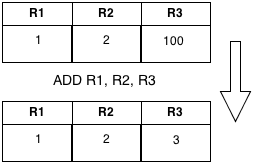
\includegraphics[scale=0.65]{images/register-based-addition.png} 
\caption{The addition of two integers on a register based virtual machine.}
\label{fig:register-based-addition}
\end{center}
\end{figure}
This minimal example shows how the register based virtual machine uses lesser machine instructions compared to the stack based.
The disadvantage in this is that register based machine has to store the addresses, the registers, of the operands.
Which is not necessary at a stack based machine, because of the stack pointer that always directs to the actual operand using the Last In First Out (LIFO) principal.
This leads to the result, that stack based code is smaller than the corresponding register based code.
Although the Dalvik VM is a register based virtual machine, the executed byte code is not bigger than the equivalent JVM code.~\cite{shi2008virtual}\\
This is the result of the different format of the executable virtual machine code, which is illustrated in Chapter~\ref{sec:comparison-of-the-two-bytecode-formats}.
\\
The performed instructions which are executed on Dalvik VM are called bytecode.
To execute this instructions the DVM has an interpreter which interprets all instructions and performs them.
The difference to normal interpreted languages is, that the JVM interpreter do not need to check the syntax of the program.
This has been already done by the Java compiler which compiles the Java source code into class files.
Even if it is faster than other interpreted languages, it is still slower than compiled code which is executed directly on the hardware.
This so called machine code is faster because there is no layer between the executions and the hardware, which could slow down the execution.~\cite{aycock2003brief}
There is a technique which can improve a virtual machine in performance aspects by adding a Just In Time (JIT) compiler to it.
Generally it can be said, that a JIT compiler, used by a virtual machine, compiles heavy used code segments or very expensive calculations into the faster machine code.
There is a great number of different types of JIT compilers and how they work, the two used by the JVM and the DVM are:
\begin{itemize}
\item method-based
\item trace-based
\end{itemize}
The trace-based method works by looking at the most executed code fragments, especially loops, and compiles them into native machine code.\\
The method-based JIT mechanism is to compile whole methods, which are often used and expensive in execution time.
Since the release of the Android version 2.2, release name Froyo, the Dalvik VM has received a JIT compiler additionally to the interpreter mechanism.
According to \cite{cheng2010jit} the implemented Dalivk JIT compiler can speed up the execution of intensive operations up to five times.
The Dalvik VM uses the above mentioned mechanism of a trace-based JIT compiler mixed with the usual DVM interpreter.
The given advantage of the trace-based method is that not whole methods are being compiled into machine code.
Instead only the parts which are often executed are being compiled.
This reduces the size of the code which needs to be compiled by the JIT and also omits the not so often executed methods parts like exception handling.
It is needles to compile such parts in machine code to speed them up, because most of the execution time of the program they were not called.
It should also reduce the compile time for the JIT because of the selective compilation into machine code.\\
To realize this the DVM has received an additional thread, which is responsible for the JIT compilation.
Beneath this new thread there is the main thread, that includes the interpreter.
This interpreter interprets the bytecode and records the traces and their occurrence.
If the amount of the occurrence higher than a predefined number, the trace is being stored into the trace queue.
The new added thread, the JIT thread, compiles the traces from the queue and writes the machine code into the code cache.
The main thread now is doing a lookup if the bytecode that needs to be executed is now available in the code cache.
Is this condition met, it uses the machine code from the code cache instead interpreting the bytecode.\cite{oh2012evaluation}
Picture~\ref{fig:dvm-threads} illustrates the principle of the two threads in the DVM.\\
\begin{figure}[h]
\begin{center}
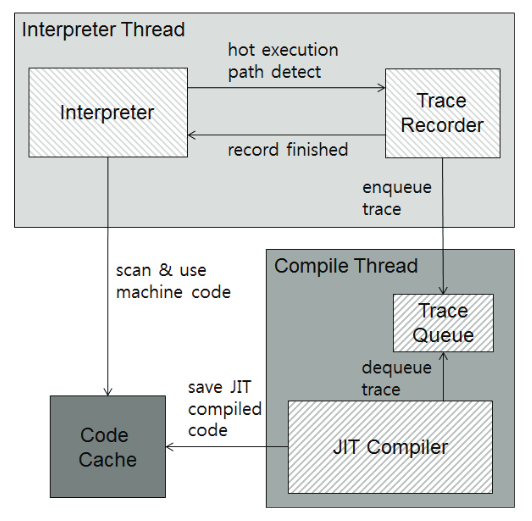
\includegraphics[scale=0.5]{images/dvm-threads.png} 
\caption{The principle of the two DVM threads. Source:\cite{oh2012evaluation}}
\label{fig:dvm-threads}
\end{center}
\end{figure}

Depending on the different implementation of a JVM, it differs which type of JIT compiler mechanism is used.
For this thesis the Oracle JVM HotSpot is used, which has a method-based JIT compiler as default.
It is also possible to use another JIT mechanism in the HotSpot JVM triggered by parameters during the VM start.
The method-based JIT works like above mentioned, it compiles the most called methods into machine code.~\cite{kotzmann2008design}
Those methods are called hot spots, which are also named the virtual machine.
\cite{paleczny2001java}
\\
Although both virtual machines are using Java as programming language, Dalvik lacks of some libraries that are available at the JVM and vice versa.
In Section~\ref{sec:migration:migration-of-basex-to-android} the used libraries of BaseX are analyzed and investigated which of them are supported by the DVM.\\
A general statement about the both virtual machines could not be made, because they differ in a lot of aspects.
Especially that the DVM has been created for the mobile context and can only be ran on Android devices\footnote{There exist some community projects which are aiming to port the Dalvik VM to other platforms like Linux x86 for example\url{http://www.android-x86.org/}}.


\subsection{Comparison of the two bytecode formats}
\label{sec:comparison-of-the-two-bytecode-formats}
Both virtual machines differ in their format of the executable files.
This is on one side the Java Archive File (JAR) for the JVM and the Davlik Executable (DEX) on the other side.
This DEX is being packed into an Android Application package file (APK) which can be executed by the Android operating system.
A JAR file is an archive which includes the compressed class files, this class files are being build out of the Java source code by using the javac compiler.~\cite{pugh1999compressing} 
An APK file is also an archive file, but it not only includes the executable program, it also includes the meta information and resource files.
The executable which includes an APK is called DEX file, which is short for Dalvik Executable.
A DEX file is created by using a tool which compiles Java class files into DEX files.
This works by a tool which is called dx and is part of the Android software development kit.
Picture~\ref{fig:create-apk} illustrates the flow of an APK creation, which differs to the creation of a JAR file by creating dex files out of the class files.\\
\begin{figure}[h]
\begin{center}
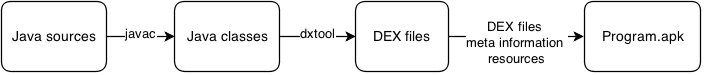
\includegraphics[scale=0.55]{images/create-apk.png} 
\caption{The creation flow of an APK file.}
\label{fig:create-apk}
\end{center}
\end{figure}

Having a closer look at the DEX files and comparing them to the JAR files shows that they differ in various ways.
The first thing that comes in mind is that a JAR file contains a class file for every class.
And a DEX file combines all specific information into one field.
Which results in that it just has one constant pool, where all constant values of all classes are stored.
These constants are:
\begin{description}
  \item[string\_ids] Sorted list of all string identifiers
  \item[type\_ids] Sorted list of all identifiers of classes, arrays or primitive types
  \item[proto\_ids] Sorted list of all prototypes
  \item[field\_ids] Sorted list of all identifiers for the used fields
  \item[methods\_ids] Sorted list of all methods used by the DEX file
\end{description}
Thinking about an interface which is used very often in a project can display what an advantage of one shared constant pool gives.
Looking at Image~\ref{fig:jar-dex} demonstrates that every class which uses this interface needs has its own reference in its own constant pool.
\begin{figure}[h]
\begin{center}
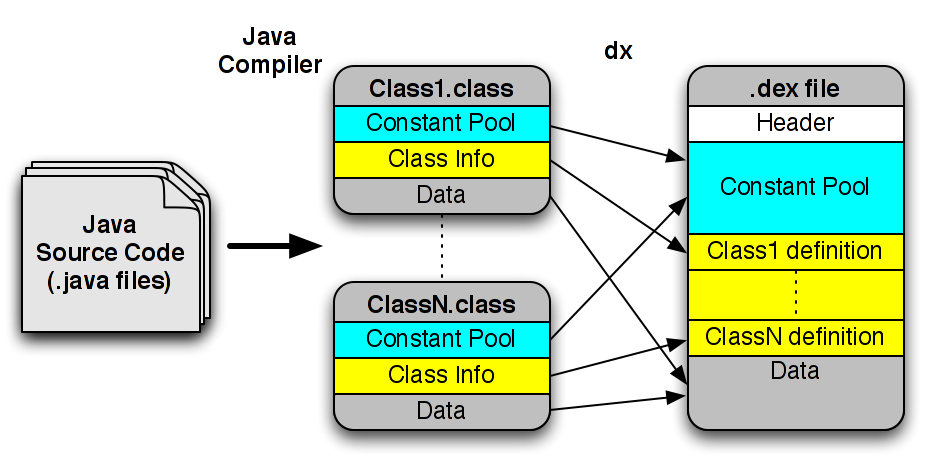
\includegraphics[scale=0.41]{images/jar-dex.png} 
\caption{The difference between a jar and a dex file. Source:~\cite{enck2011study}}
\label{fig:jar-dex}
\end{center}
\end{figure}

In general it can be said that DEX files are smaller than their equivalent JAR files, because of the shared constant pool.~\cite{bornstein2008dalvik}
An advantage of the creation chain of a DEX file is that it is theoretically possible to create a DEX file out of every jar archive.
The problem hereby is that Android does not support all Java libraries that the JVM supports, but this can be done by using the above mentioned dx-tool. 
Like mentioned above this DEX file is executed by the Dalvik virtual machine, but it is not the Android application.
This application is the APK  which includes also UI related information and other resource files, like images or sound.


\subsection{Android internals}
\label{sec:android-internals}
As shown in the Sections~\ref{sec:migration:comparison-of-the-two-virtual-machines} and \ref{sec:comparison-of-the-two-bytecode-formats} the two virtual machines and the bytecode formats differ.
However, Android has some other specialties about its internal processing.
The Android operating system is a Linux based operating system aimed to run on mobile devices.
Therefore it has been created as a Linux fork of the 2.6.*\footnote{Since Android version 4.* a Linux kernel 3.* is used} kernel and 
It is being especially designed for the mobile context.
Which includes special focus for the resource consumption, because most mobile devices provide not the same resources as a normal desktop PC or a notebook.
As shown in Section~\ref{sec:migration:comparison-of-the-two-virtual-machines} an Android application is executed on the Dalvik virtual machine.
Here it need to be said that every application runs its own Dalvik instance, by forking the main Dalvik instance into an own Linux process.
Here sets the Android policy in, that every application is independent from every other application and is executed in its own process.
This also is applied for the location of all files the application uses.
An application can be compared as an user in Linux, every application is its own user and has its own home directory.
This directory can only be accessed by the owning application and can be found in the /data/data directory.
This directory includes an own SQLite3 database, cache directory, shared preferences\footnote{Android framework that provides a mechanism to store primitive data types.} and every type of private data.
A reason for this is a security aspect as well as the stability of the application, considering the own Dalvik instance.
This is called the \textit{principle of least privilege} which specifies that as less as possible privileges are given to the application.
Therefore an application developer has to specify which privileges its application needs, for example Internet access or the possibility to write on the external SD-card.
It is possible that applications can communicate with predefined Inter Process Communications (IPC) but it is not possible to manipulate other applications.
This can be omitted by granting an application root privileges, but usually this is not possible on normal devices.
Hence, confidential data should also be encrypted,because it is theoretically possible to access the data in the private directory.
It also need to be mentioned that every operation which reads or writes to on of the above mentioned directories or files is an input output (IO) operation.
This is always expensive in time consumption and should be done as little as possible.
Image~\ref{fig:zygote-and-app} illustrates the principle that every application works in its own sandbox.\\
\begin{figure}[h]
\begin{center}
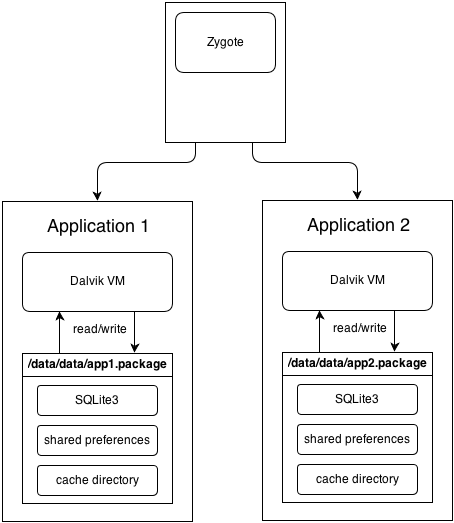
\includegraphics[scale=0.65]{images/zygote-and-app.png} 
\caption{Illustration of the Android application architecture}
\label{fig:zygote-and-app}
\end{center}
\end{figure}
The main Dalivk instance which is the root for all forked virtual machines is called Zygote and is started by the boot up process.
Zygote is designed to load and initialize the core library classes so that every forked instance do not have to do this.
This is compared to starting a new virtual machine a speed improvement and saves memory, because not every VM instance has its own core libraries loaded.
This can be done because the core libraries are all read only and shared by all Dalvik instances.\cite{ehringer2010dalvik}
Another difference to the usual Linux is that Android uses Bionic libc which is a special from Google developed library for Android which has its own pthread implementation.
This library is especially designed for the mobile context and the Android environment which improves the speed of forking the Dalvik virtual machine too.~\cite{brady2008android}
\newpage
\section{Migration of BaseX to Android}
\label{sec:migration:migration-of-basex-to-android}
After analyzing both platforms the BaseX database code need to be examined too.
Like it has been mentioned in Section~\ref{sec:migration:comparison-of-the-two-virtual-machines} the Dalvik virtual machine does not support all class libraries that are supported by the JVM.
BaseX is written in the Java programming language and aims to be executed on virtual machines that are implemented by using the JVM specifications.
Therefore it is not possible to transform the BaseX jar file into a DEX file, using the dx-tool, and execute it on an Android device.
On the other side the DVM offers class libraries that the JVM does not support or knows.
These libraries do not intent to replace not supported Java class libraries, there purpose is to provide special Android related methods, for example logging or tracing of method calls.

\subsection{Analyzing the libraries used by BaseX}
\label{sec:migration:analyzing-the-libraries-used-by-basex}
BaseX is a big project which includes up to 60 packages and more than 1300 classes, interfaces and abstract classes.
For this reason the examining of the used libraries and the dependencies a tool was used.
It is called Class Dependency Analyzer (CDA)\footnote{http://www.dependency-analyzer.org/} and offers all needed possibilities for the mentioned task.
Parsing the whole BaseX project lists the used Java class libraries and external libraries.
This list gives 54 packages that are part of the Java class library or an external library used by BaseX.
It has to be supposed that none of them are known to the Dalvik virtual machine.
Most of them are subpackages of packages and it can be expected that if a main package is not supported by Android the subpackage also not. 
This assumption reduces the external packages to a number of 16, which is compared to the before mentioned 54 packages an easier to analyze amount.
Looking at the Android documentation the main packages that are not supported are just the two GUI related packages.
\begin{itemize}
  \item java.awt\footnote{except the subpackage java.awt.font that provides two classes: NumericShaper and TextAttribute.}
  \item javax.swing
\end{itemize}
All others are full or partially supported by the Dalvik VM.
The reason why the packages awt and swing are not supported is that Android uses its own GUI libraries.
laber something über android ui bla blub

\newpage





For the migration an Android project has been created, this provides all needed files.
To create an Android project the Android Software Development Kit(SDK) is necessary.
This can be downloaded on the official homepage of Android\footnote{\url{developer.android.com/sdk/index.html}}
The Android SDK, which is also called Android Developer Tools(ADT), provides many useful tools and also a plugin for the Eclipse IDE.
To create the BaseX library project the Eclipse create new project wizard has been used.
It is possible to mark the project as a library, this implies that the compiler creates a jar file out of the project.
The purpose of this is that the BaseX library can be used in every Android project by just including it.
All private data is stored in the /data/data/packagename directory.
So the method not just only creates an instance or returns the existing, it also checks if the private folder of the application is available and creates it if not.
If this folder has been created there is also a subfolder created which is called BaseXData.
This subfolder stores all databases created by the application and no other application can neither read nor write on this folder.
The next necessary change is to adjust the path on the Prop.java file.
This contains a static class that holds every property of the BaseX database, hence also the path to the database.
This has to be done before anything can read the filepath, so it is part of the constructor call.
BaseX provides methods that can be used to access, create, modify or delete the database.
For every of these operations a method inside the class has been created and can be called from outside.
Every method checks if a BaseX context is available, which should usualy be the case, and then executes the wanted operation.
Therefore the BaseX context is necessary and is used to make the specific operation on the database.
Every method in the class throws an IOException when something goes wrong, this exception comes from BaseX and need to be handled by the application which uses the library.
The reason why the directory name of the application has to be used at the constructor call is that it is not possible to get the name of the application inside the library.
There are methods provided by Android to receive the project package name, but this is the name of the package of the library.
And the library is not an application and therefore has no own data directory in the /data/data folder.
And it is not possible to create a own folder in this directory, because Android is doing it when the Application is being installed.
It would be also always the same folder, because 



%Android uses a different kind for generating UI objects than the standard Java version.
%This uses AWT and Swing, but these API aren't available on Android, so this can not be used on Android.
%Another difference between Android and the standard BaseX version is that Android has no user directory.
%Every application has its own directory which is located in /data/data/packagename.
%Therefore all files need to be stored there. 
%BaseX Android should be a library which means that every developer can use it.
%Therefore it is not known how the absolute path name is, because it is the package name of the executing activity.
%And this name differs from project to project.
%Therefore there is just one entry point for the library which is the class BaseXAndroid.
%The constructor of this class has a string argument, this parameter should be the absolute path to data directory of the application.
%To get this needed information the function getApplicationInfo().dataDir, which is inherited from the activity class, can be used in every activity of the application.




\section{Problems during the migration}
\label{sec:migration:problems-during-the-migration}
There occurred several problems during the migration.
The first problem which was discovered, was that some included libraries are not available on Android.
The following library couldn't be migrated because it is included in the JavaSE and is not available for Android.
\textit{crypto javax.xml.crypto}
BaseX identifies the operating system as Linux and then tries to save all BaseX related data into the home directory, which doesn't exist on Android.
This need to be, like in Section~\ref{sec:migration:requirmenets-of.the-target-platform} described the /data/data/application directory.
The problem hereby is that the goal of the migration is that the database is a library, but the directory name depends from the application name.
The only way to get the application way, except for hard coding, is to get the application context and extract the name there.
This bears another problem, though only applications have a context, libraries not. 
A possible way, could be to pass the context to the library, but then the library holds the context and just need to application name.
Holding a context massively slows down an Android application, so this is not the way how it was solved.
The alternative is to pass a string holding the application name to the library constructor and the library uses it to generate the needed directories.
This is also the way how it is done in the BaseX library.
To create a library object it is necessary to pass a string as an argument to the constructor.
Is this the first time an object of BaseX was created it tries to create the needed directory, /data/data/application-name/BaseXData.
In this directory all created databases and their depending files are stored.
\\
Another problem which occurred, was that BaseX uses a lot of the String function isEmpty(), which is not available at API-Level lower than 9.
The same applies for the copyOf() method in the java.util.Arrays package.
This was solved by not supporting API-level lower than 9 with BaseX library. 
The reason for this is that only 4\% of the used Android devices are using API-level lower than 9.
\\
After this adjustments it is possible to create a BaseX object on Android.
To get a library which supports all needed operations some more work was done.



